\section{Experimental Setup}
\label{sec:experiment}
\subsection{Models and Inputs}
We test the three models in \cref{tab:model-inputs}. Each one accepts text, images, and text and image together \citep{embeddinggemma2_modelcard,qwen3vl_embedding_modelcard,gme_modelcard}. We use each model as released, at its full embedding size, and normalize every embedding to unit length. Qwen3-VL and GME share Qwen ancestry, so these are three models rather than three unrelated architectures. Exact versions, prompts, and preprocessing are given in \cref{app:embedding-protocol}.

\begin{table}[t]
\centering
\caption{The three models and their inputs. Image: size after the model's own resizing (EmbeddingGemma 2 always uses 280 image tokens). Text tokens include the model's prompt template (sample 0 of all 54 problems). Last column: average CPU seconds per text/image/joint input (bfloat16, two cores).}
\label{tab:model-inputs}
\small
\setlength{\tabcolsep}{3pt}
\resizebox{\columnwidth}{!}{%
\begin{tabular}{lcccc}
\toprule
Model & Dim. & Image & Text tokens & s/input \\
\midrule
EmbeddingGemma 2 & 768 & 280 tok. & 454--921 & 0.4/1.9/2.3 \\
Qwen3-VL-Emb.-2B & 2,048 & $704\times288$ & 447--912 & 1.5/1.6/2.8 \\
GME-Qwen2-VL-2B & 1,536 & $728\times308$ & 447--912 & 1.5/2.7/4.1 \\
\bottomrule
\end{tabular}}
\end{table}


Each model receives three kinds of input: the text description, an image of the solution, and both together. For the joint input we use the model's own interface for combined text and image; averaging a text embedding and an image embedding would be a different method. The same prompt and preprocessing are used for every input of a given kind.

The image is a single $688\times286$ picture of five snapshots: one row per field and one column per observed time (\cref{fig:configurations}; a real example is in \cref{app:extra}). Each $64\times64$ field is enlarged by repeating pixels and colored with the viridis colormap on the fixed range $[0,0.8]$, chosen from the pilot. No image is rescaled on its own, and the underlying arrays are never changed. The only text in the image is the five time labels and the field names $u$ and $v$.

\begin{figure}[t]
\centering
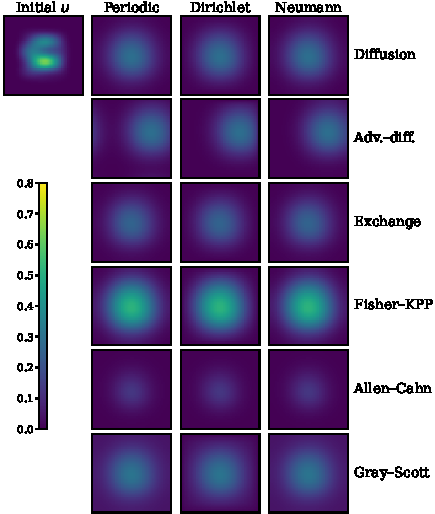
\includegraphics[width=0.94\columnwidth]{figures/fig_configurations.pdf}
\caption{The 18 problems that share one initial field (oscillation family, sample 1): $u$ at $t=1$ for six equations and three BCs, on a common color scale. Because the initial data vanish near the boundary and the horizon is short, the BC changes the solution much less than the equation does.}
\label{fig:configurations}
\end{figure}

\subsection{What We Ran and How We Score It}
All 5,400 trajectories, the reference distances, and the model-free baselines use all 100 samples. Running the three models on all 48,600 inputs was not possible on the two-core CPU we had (\cref{tab:model-inputs}). Before encoding any test input, we therefore fixed a smaller set: samples 0--9 of all 54 problems for the main runs (1,620 inputs per model), and samples 0--2 for the controls. Each model is always compared with the reference computed on the same samples. On these ten samples the reference rankings are almost identical to those from all 100 samples (mean Spearman correlation \refSubsetVsAll{}).

Within each IC family there are 153 pairs of distinct problems. Our main score is the Spearman rank correlation between the model similarity $S^{\mathrm{emb}}$ and $-D$ over these pairs, averaged over the three families. The second score is \emph{triplet accuracy}. Take an anchor problem and two others; if the reference says the first is closer to the anchor, does the model agree? Exact ties in the reference are skipped, and ties in the model count as one-half. We also split the pairs into those with the same BC and those with different BCs. The $54\times54$ matrix and the 100-frame reference are secondary.

Numerical error is far too small to affect these rankings. The error bound $\epsilon_i$ of \cref{prop:margin} is at most \refEpsLinear{} for the linear equations, where we compute it from exact solutions. For the nonlinear equations it is at most \refEpsNonlinear{}, estimated by refining the time step, with a safety factor of two. Reference distances range from \refDmin{} to \refDmax{}. All 7,344 triplets within IC families pass the test of \cref{prop:margin}, and the 10.3\% that involve only linear equations are proved up to rounding. Grid resolution matters just as little: on pilot samples, moving to a $128\times128$ grid changed the order of \pilotFlips{} of \pilotTriplets{} triplets (\cref{app:pilot}).

For uncertainty, we resample the ten samples with replacement (2,000 times), recompute both matrices, and report 95\% intervals. These intervals reflect the random ICs, not the choice of equations or BCs, and with ten samples they are rough. The pairs in a matrix are not independent, and nothing here supports claims about PDE families we did not test.

\subsection{Baselines and Controls}
\paragraph{Baselines.}
For text we use character 3--5-gram TF--IDF. For images we compare the raw pixels and, separately, the magnitudes of the low spatial Fourier modes ($|k|\le8$ in each direction). The physical cosine of \cref{sec:comparison} shows how well shape alone, without size, predicts the reference. The RMS distance on the numbers themselves is the reference, so it is not a baseline.

\paragraph{Initial frame only.}
An image showing only $t=0$ is the same for all 18 problems in an IC family. If a model is deterministic, all its similarities within a family equal one, the Spearman correlation is undefined, and triplet accuracy is $0.5$. This is the floor for a model that sees only the starting state.

\paragraph{Time order.}
We reverse the five snapshots in every image but leave the time labels in place. Reordering frames in the same way for every problem does not change the reference, so a model that responds to the fields themselves should give similar rankings.

\paragraph{Notation.}
We rewrite each description in an equivalent form: the Laplacian becomes second derivatives, diffusion moves to the end of each equation, and the coordinates $x,y$ become $\xi,\zeta$ in every formula. The rewritten problem is mathematically identical. Separately, four short heat-equation descriptions differ only in the diffusion coefficient of \cref{tab:calibration}.

\paragraph{Mismatched inputs.}
We pair the image of each problem with the description of the next equation in our list, keeping the same IC, BC, and sample. We then ask whether the joint similarities follow the reference for the image or the reference for the text.
